\documentclass[letterpaper,10pt,serif, draftclsnofoot,onecolumn, compsoc, titlepage]{IEEEtran}

\usepackage{graphicx}
\usepackage{amssymb}
\usepackage{amsmath}
\usepackage{amsthm}

\usepackage{alltt}
\usepackage{float}
\usepackage{color}
\usepackage{url}

\usepackage{balance}
\usepackage[TABBOTCAP, tight]{subfigure}
\usepackage{enumitem}
\usepackage{pstricks, pst-node}

\usepackage{geometry}
\geometry{margin=.75in}

\usepackage{hyperref}

% This method for displaying a relational schema was found on Stack Exchange from user Bruno Vandekerkhove
% tex.stackexchange.com/questions/296948/creating-a-relational-database-schema
\usepackage{tikz}
\usetikzlibrary{shapes, positioning, calc}
\colorlet{lightgray}{gray!20}

\begin{document}

% Adding these from the template in Annex C of the standard
% Some may not apply, but I'm sure most will
\section{Kyle- Database Management}
\subsection{Database organization}

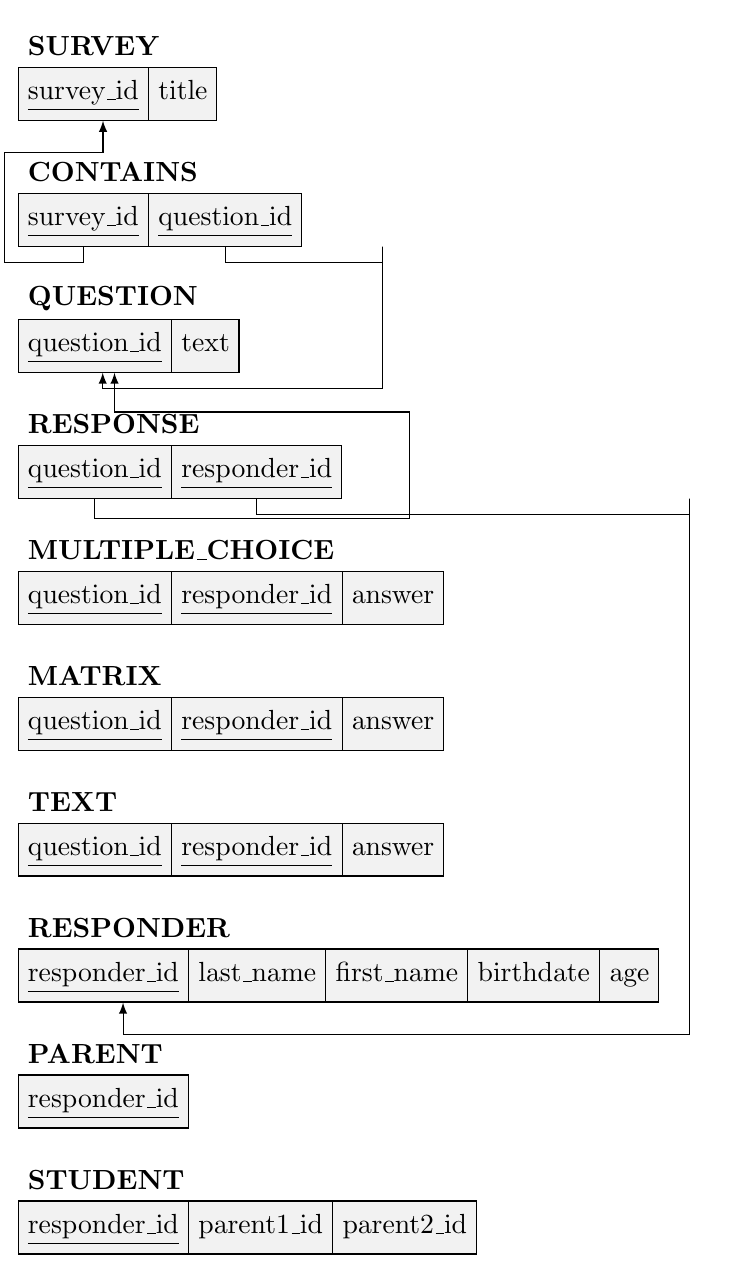
\begin{tikzpicture}[relation/.style={rectangle split, rectangle split parts=#1, rectangle split part align=base, draw, anchor=center, align=center, text height=3mm, text centered}]\hspace*{-0.3cm}

% Relations

\node (surveytitle) {\textbf{SURVEY}};
\node [relation=2, rectangle split horizontal, rectangle split part fill={lightgray!50}, anchor=north west, below=0.6cm of surveytitle.west, anchor=west] (survey)
{\underline{survey\_id}%
\nodepart{two}		title};

\node [below=1cm of survey.west, anchor=west] (containstitle) {\textbf{CONTAINS}};
\node [relation=2, rectangle split horizontal, rectangle split part fill={lightgray!50}, anchor=north west, below=0.6cm of containstitle.west, anchor=west] (contains)
{\underline{survey\_id}
\nodepart{two}	\underline{question\_id}};

\node [below=1cm of contains.west, anchor=west] (questiontitle) {\textbf{QUESTION}};
\node [relation=2, rectangle split horizontal, rectangle split part fill={lightgray!50}, anchor=north west, below=0.6cm of questiontitle.west, anchor=west] (question)
{\underline{question\_id}%
\nodepart{two}		text};

\node [below=1cm of question.west, anchor=west] (responsetitle) {\textbf{RESPONSE}};
\node [relation=2, rectangle split horizontal, rectangle split part fill={lightgray!50}, anchor=north west, below=0.6cm of responsetitle.west, anchor=west] (response)
{\underline{question\_id}%
\nodepart{two}		\underline{responder\_id}};

\node [below=1cm of response.west, anchor=west] (multiplechoicetitle) {\textbf{MULTIPLE\_CHOICE}};
\node [relation=3, rectangle split horizontal, rectangle split part fill={lightgray!50}, anchor=north west, below=0.6cm of multiplechoicetitle.west, anchor=west] (multiplechoice)
{\underline{question\_id}%
\nodepart{two}		\underline{responder\_id}
\nodepart{three}	answer};

\node [below=1cm of multiplechoice.west, anchor=west] (matrixtitle) {\textbf{MATRIX}};
\node [relation=3, rectangle split horizontal, rectangle split part fill={lightgray!50}, anchor=north west, below=0.6cm of matrixtitle.west, anchor=west] (matrix)
{\underline{question\_id}%
\nodepart{two}		\underline{responder\_id}
\nodepart{three}	answer};

\node [below=1cm of matrix.west, anchor=west] (texttitle) {\textbf{TEXT}};
\node [relation=3, rectangle split horizontal, rectangle split part fill={lightgray!50}, anchor=north west, below=0.6cm of texttitle.west, anchor=west] (text)
{\underline{question\_id}%
\nodepart{two}		\underline{responder\_id}
\nodepart{three}	answer};

\node [below=1cm of text.west, anchor=west] (respondertitle) {\textbf{RESPONDER}};
\node [relation=5, rectangle split horizontal, rectangle split part fill={lightgray!50}, anchor=north west, below=0.6cm of respondertitle.west, anchor=west] (responder)
{\underline{responder\_id}%
\nodepart{two}		last\_name
\nodepart{three}	first\_name
\nodepart{four}	birthdate
\nodepart{five}		age};

\node [below=1cm of responder.west, anchor=west] (parenttitle) {\textbf{PARENT}};
\node [relation=1, rectangle split horizontal, rectangle split part fill={lightgray!50}, anchor=north west, below=0.6cm of parenttitle.west, anchor=west] (parent)
{\underline{responder\_id}};

\node [below=1cm of parent.west, anchor=west] (studenttitle) {\textbf{STUDENT}};
\node [relation=3, rectangle split horizontal, rectangle split part fill={lightgray!50}, anchor=north west, below=0.6cm of studenttitle.west, anchor=west] (student)
{\underline{responder\_id}%
\nodepart{two}		parent1\_id
\nodepart{three}	parent2\_id};

% Foreign keys

\draw[-latex] (contains.one south) -- ++(0,-0.2) -| ($(contains.one south) + (-1,0)$) |- ($(survey.one south) + (0.25,-0.40)$) -| ($(survey.one south) + (0.25,0)$);

\draw[-latex] (contains.two south) -- ++(0,-0.2) -| ($(contains.two south) + (2,0)$) |- ($(question.one south) + (0.25,-0.20)$) -| ($(question.one south) + (0.10,0)$);

\draw[-latex] (response.one south) -- ++(0,-0.25) -| ($(response.one south) + (4,0)$) |- ($(question.one south) + (0.25,-0.50)$) -| ($(question.one south) + (0.25,0)$);

\draw[-latex] (response.two south) -- ++(0,-0.2) -| ($(response.two south) + (5.50,0)$) |- ($(responder.one south) + (0.25,-0.40)$) -| ($(responder.one south) + (0.25,0)$);

\end{tikzpicture}

\end{document}